\section{Predicting Building Pressurization}

Building pressurization can be used as an effective ITS under the right circumstances.
However, determining this requires a measurement device to be installed, and moreover needs to record over some length of time to determine trends.
Thus, it would be desirable to use some more readily available metric, such as weather data, to predict building pressurization.\par

A variety of factors can contribute to determine overall building pressurization.
Some of these are artificially controlled and induced, such as the force convection by heating, ventilation, and air conditioning systems.
These are of course difficult to use to for prediction purposes, and can at some sites be the dominant means for controlling building pressurization, i.e. some buildings or rooms are forcefully pressurized to keep gases or contamination out.\par

Weather primarily contributes to building pressurization through two means.
The temperature difference between the interior of the building produces a density and subsequent pressure gradient on either side of the building wall - this is commonly called the \textit{stack effect}.
Wind striking the building also produces a pressure difference, the magnitude of which is largely dependent on wind speed.
However, if the building is pressurized or depressurized by this, is more complicated and generally depends on the wind direction and building characteristics; wind blowing on a leaky window causes a very different effect compared to a featureless wall.\par

These weather phenomena likewise can affect air exchange rates, and has been a significant focus in the VI modeling work by \citeauthor{shirazi_three-dimensional_2017}\cite{shirazi_three-dimensional_2017}.
As their work shows, predicting air exchange rate can be challenging, as accurate characterization often require detailed knowledge of the interior of a building, and will not be a focus in this work.\par

\subsection{Wind Effects}

To truly capture the impact that wind can have on a building and its pressurization, it is usually necessary to conduct wind tunnel tests of scale models of the building, or through detailed computational fluid dynamics simulations.
This is especially true for buildings of even modest complex geometric shapes, where it is impossible to predict the wind pressure field without these tools.
However, it is possible to derive some simple equations to account for wind effects on simple rectangular block-type buildings.\par

Even with assumption, the inherent turbulent nature of wind means that is truly never at steady-state, and thus wind striking a wall generates a distribution of pressures across the surface, that can vary widely across time; this requires significant computational effort to resolve accurately.
However, by considering the wind induced pressure field over some time-averaged period, it is possible to develop some simple equations for predicting wind induced pressurization for a rectangular building.
The drawback of this approach is that large pressure fluctuations are usually missed.\par


Wind is also inherently turbulent, and as such it is never truly at steady-state.
Thus, wind pressure as it strikes the wall of a building can fluctuate wildly





With these limitations in mind, we introduce some equations for estimating wind induced building pressurization.

As the wind strikes the wall of a house, its velocity falls to zero, and the change in momentum is directly proportional to the change in pressure:
\begin{equation}\label{eq:wind_pressure_uncorrected}
  \Delta P = \frac{1}{2} \rho_\mathrm{air} u_\mathrm{wind}^2
\end{equation}
where $\Delta P = P_\mathrm{wall} - P_\mathrm{wind}$ [\si{\pascal}] is the change in pressure at the building wall from the wind free-stream pressure;
$\rho_\mathrm{air}$ [\si{\kilo\gram\per\metre\cubed}] is the air density;
and $u_\mathrm{wind}$ [\si{\metre\per\second}] is the free-stream wind speed.\par

However, \eqref{eq:wind_pressure_uncorrected} neglects a variety of factors, such as the obstacles in front of the surface (e.g. vegetation or other buildings), or wind striking the surface at an angle.
These can be accounted for by introducing a drag or pressure coefficient $C_p$, which is, using the same notation as in \eqref{eq:wind_pressure_uncorrected}, defined as:
\begin{equation}
  C_p = \frac{\Delta P}{\frac{1}{2} \rho u^2_\mathrm{wind}}
\end{equation}
$C_p$ values are usually determined empirically in wind tunnel tests, or by solving the Navier-Stokes equation in some computational fluid dynamics simulation.\par

Introducing the $C_p$ correction then gives
\begin{equation}\label{eq:wind_pressure}
  \Delta P = C_p \frac{1}{2} \rho_\mathrm{air} u_\mathrm{wind}^2
\end{equation}


\subsection{Temperature Effects}

The pressure of any fluid under the influence of gravity varies with elevation and the density of the fluid determines the magnitude of this pressure.
Air is a compressible fluid and its density depends on its temperature.
Therefore, if you separate two air masses between a wall, with each at a difference temperature, a pressure difference across the wall be induced, i.e. the \textit{stack effect}.

Assuming the ideal gas law applies and that the temperature on either side is constant then
\begin{equation}
  P = P_0 \exp{\Big( \frac{-M_\mathrm{air}gz}{RT} \Big)}
\end{equation}
determines the pressure variation across the wall.
Where $P$ is the pressure;
$P_0$ the reference pressure ($z=0$);
$M_\mathrm{air}$ is the molar weight of air;
$z$ is the elevation;
$g$ is the acceleration due to gravity;
$R$ is the gas constant;
and $T$ is the temperature.\par

This can be further simplified by defining $z_0$ which is the height at which the pressure on both sides of the wall are equal, i.e. $P_0$.
The pressure variation on either side can now be expressed in terms of distance from $z_0$, $z-z_0$.
Assuming that the interior and exterior has a constant temperature of $T_i$ and $T_o$ respectively, the difference in pressure between the two sides along the wall is
\begin{equation}
  \Delta P = P_0 \Big[ \exp{\Big( \frac{-M_\mathrm{air}g(z-z_0)}{RT_i} \Big)} - \exp{\Big( \frac{-M_\mathrm{air}g(z-z_0)}{RT_o} \Big)} \Big]
\end{equation}
Using that $e^{-x} = 1 - x$ for $x \ll 1$ the pressure difference can be expressed as
\begin{equation}
  \Delta P = \alpha \Big( \frac{1}{T_o} - \frac{1}{T_i} (z-z_0)\Big)
\end{equation}
where $\alpha = \frac{P_0 M_\mathrm{air} g}{R} \approx 3454 \SI{3454}{\pascal\kelvin} \; \mathrm{ \frac{Pa \cdot K}{m}Pa}$.
Here a negative pressure differnece, $\Delta P < 0$, indicates an inward flow.\par

% Is P0 the barometric pressure?

\subsection{Heating, Ventilation And Air Conditioning}


\subsection{Predicting Pressurization At The EPA Duplex}

The equations for predicting $p_\mathrm{in}$ as a function of temperature and wind are applied to the weather data from EPA duplex, and



\begin{figure}[htb!]
  \centering
  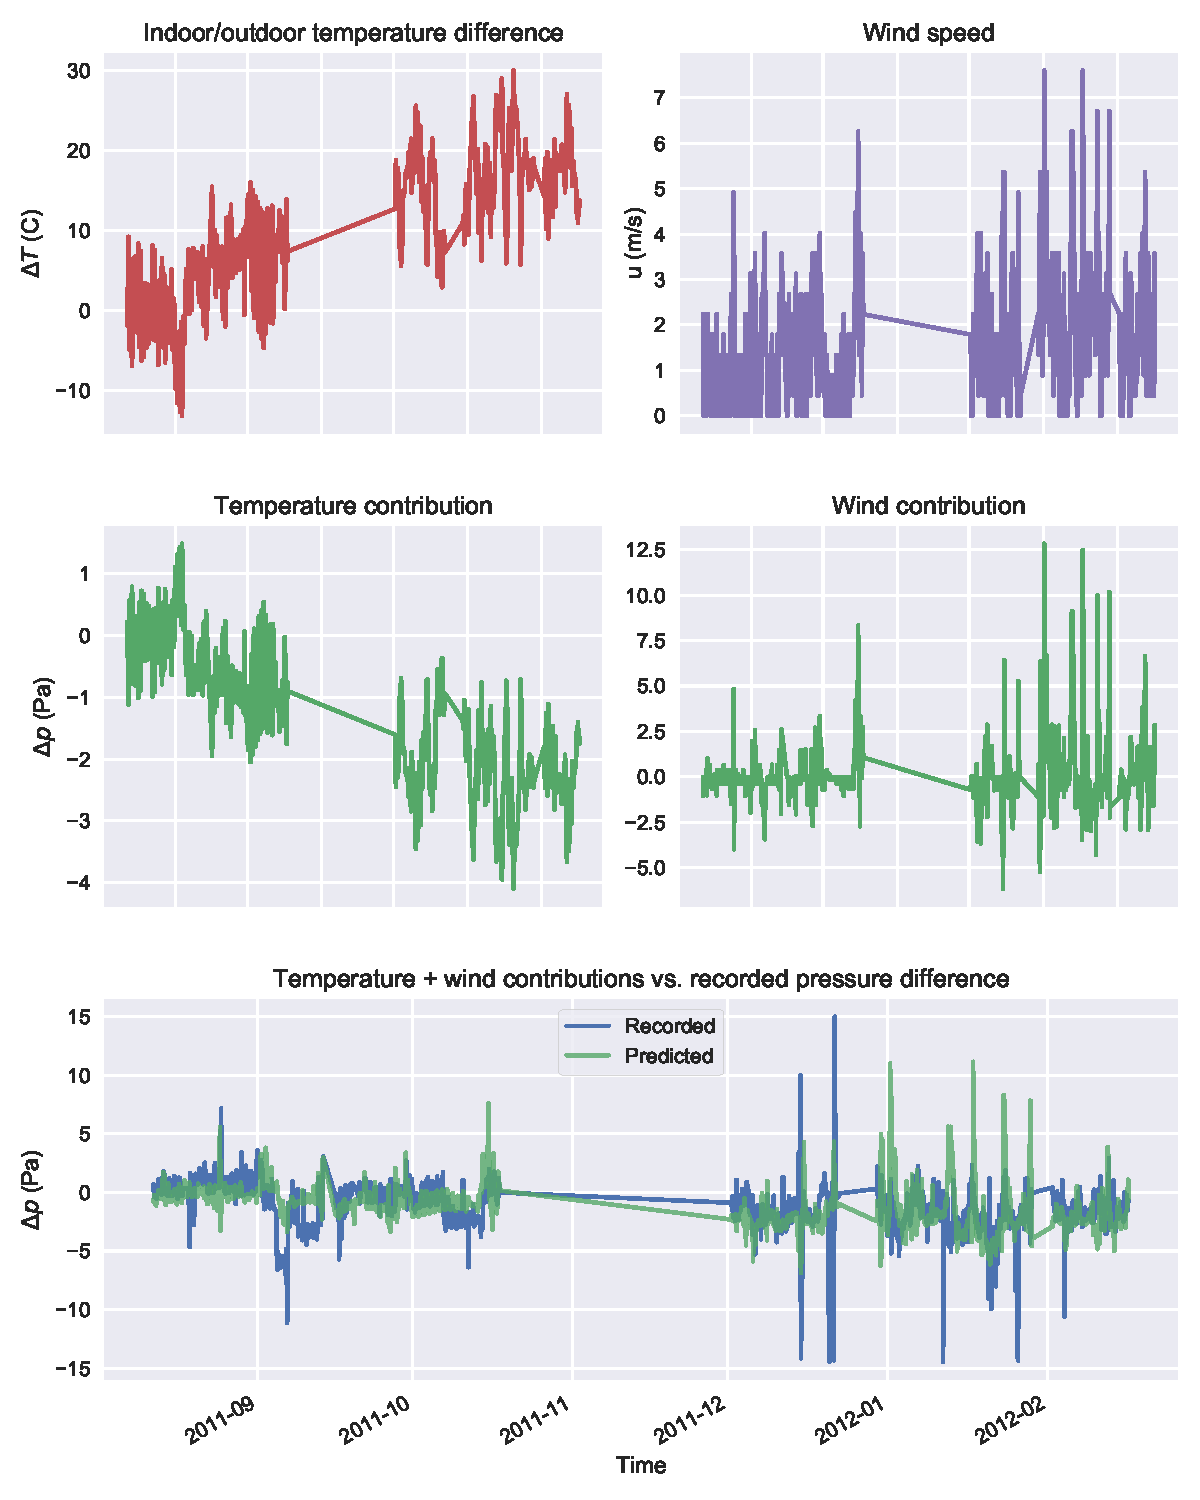
\includegraphics[width=\textwidth]{pressure_prediction.pdf}
  \caption{TBD}
  \label{fig:pressure_prediction}
\end{figure}


\begin{table}[htb!]
  \centering
  \begin{tabular}{l c c c c}
    \toprule
    & Data & \multicolumns{3}{c}{Prediction} \\
    & & $p_\mathrm{temp}$ & $p_\mathrm{temp} + p_\mathrm{wind}$ & $p_\mathrm{temp} + p_\mathrm{wind,corr}$ \\
    \hline
    Mean & -1.33 & -1.50 & -0.83 & -1.37 \\
    Std. & 2.15 & 1.12 & 1.40 & 1.50 \\
    \bottomrule
  \end{tabular}
  \caption{}
  \label{tbl:pressure_prediction}
\end{table}
